\documentclass[SE,lsstdraft,authoryear,toc]{lsstdoc}
\input{meta}

% Package imports go here.
\usepackage{graphicx}   % for \includegraphics

% Local commands go here.
\newcommand{\lhalos}{\textsc{legacyhalos} }


%If you want glossaries
%\input{aglossary.tex}
%\makeglossaries

\title{Surface brightness profiles around massive galaxies in ComCam data}

% This can write metadata into the PDF.
% Update keywords and author information as necessary.
\hypersetup{
    pdftitle={Surface brightness profiles around massive galaxies in ComCam data},
    pdfauthor={First Last},
    pdfkeywords={}
}

% Optional subtitle
% \setDocSubtitle{A subtitle}

\author{%
First Last
}

\setDocRef{SITCOMTN-165}
\setDocUpstreamLocation{\url{https://github.com/lsst-sitcom/sitcomtn-165}}

\date{\vcsDate}

% Optional: name of the document's curator
% \setDocCurator{The Curator of this Document}

\setDocAbstract{%
Low surface brightness photometry of massive galaxies probes the extended stellar halos and intracluster light but is often limited by background‐subtraction and masking systematics. Here we present radial surface brightness profiles for the brightest cluster galaxies in Abell 360 and 2dFGRS TGS323Z113 using early Rubin Observatory Commissioning Camera (LSSTComCam) Data Preview 1 in the $g$, $r$, and $z$ bands. Our result show that the LSSTComCam data can go down to $\sim30$ mag arcsec$^{-2}$ in the $r$ band.  Comparison to DECaLS measurements processed with \textsc{Legacyhalos} shows excellent agreement at small radii while the ComCam data extend deeper at larger radii.  
}

% Change history defined here.
% Order: oldest first.
% Fields: VERSION, DATE, DESCRIPTION, OWNER NAME.
% See LPM-51 for version number policy.
\setDocChangeRecord{%
  \addtohist{1}{YYYY-MM-DD}{Unreleased.}{First Last}
}


\begin{document}

% Create the title page.
\maketitle
% Frequently for a technote we do not want a title page  uncomment this to remove the title page and changelog.
% use \mkshorttitle to remove the extra pages

% ADD CONTENT HERE
% You can also use the \input command to include several content files.

\section{Introduction}
The deep and wide photometric data provided by LSST opens significant opportunities for low-surface brightness science, but the extent to which we can push our photometry depends sensitively on the accuracy of our background modeling. In particular, there can be background over- or under-subtraction near bright sources, and large-scale backgrounds that are scientifically interesting (e.g., the intracluster light) are often removed by the default processing. The massive, central galaxies in galaxy clusters are a good test bed for these effects as they have large, extended stellar envelopes that can be traced down to low surface brightness and live in crowded fields, making the photometry in the outskirts of these galaxies particularly sensitive to the background modeling.
In this note, we focus on two relatively massive clusters in the Rubin ComCam commissioning data, Abell 360 and 2dFGRS TGS323Z113. We measure the surface brightness profiles of the central galaxies in these clusters and compare them to precursor data.

\section{Data}
The Rubin data we use in this paper is from the Data Preview 1 (DP1). DP1 data is based on the reprocessing of exposures acquired over 48 nights during the first on-sky commissioning campaign using the Rubin Commissioning Camera, LSSTComcam, between November 2024 and December 2024 \cite{ComCam}. DP1 covers 7 distinct non-contiguous fields with a total area of 15 sq. deg. Among the seven fields are the Rubin SV Low Ecliptic Latitude Field (Rubin SV 38 7), in which the galaxy cluster Abell 360 is located, and Extended Chandra Deep Field South (ECDFS), in which galaxy 2dFGRS TGS323Z113. The Rubin SV 38 7 field has a total 159 visits in g, r, i, z band,s and ECDFS has a total of 855 visits in u,g,r,i,z,y bands. 

We use the photometry measured with Legacyhalos \cite{liReachingEdgeProbing2022,moustakasSienaGalaxyAtlas2023} from Legacy Survey Data Release 9 data as a comparison. Legacy Survey DR9 data (LS DR9) \cite{schlegelDESILegacyImaging2021} is designed to provide faint extragalactic targets for the Dark Energy Spectroscopic Instrument's cosmological survey. LS DR9 includes g, r, and z-band data from Dark Energy Camera Legacy Survey (DECaLS), the Beijing-Arizona Sky Survey (BASS), and the Mayall z-band Legacy Survey (MzLS), and public data from the Dark Energy Survey (DES). In this work, we only use the data from DECaLS. The images were first processed with the NOAO community pipeline and Tractor algorithm. Then, a photometry pipeline optimized for elliptical galaxies, \textsc{Legacyhalos}, is used to measure the surface brightness profile around a set of targets. A subset of the legacyhalos measurements were compared with Hyper-Suprime Cam survey measurements and show excellent agreements in a statistical sense to $R > 200$ kpc \cite{liReachingEdgeProbing2022}. 

\begin{figure}[htbp]
  \centering
  % adjust width as you like (e.g. 0.8\linewidth, or specify height)
  \includegraphics[width=0.8\linewidth]{figures/coadd.pdf}
  \caption{r-band coadd image of the BCG of A360 and 2dFGRS TGS323Z113 }
  \label{fig:image}
\end{figure}


\section{Surface brightness profile}
In this section, we describe the method we use to extract surface brightness profiles from ComCam data. We start with the background subtracted \texttt{deepCoadd\_calexp} images in $g, r, z$ bands. We use \texttt{DETECTED} mask in each band to mask out the $5 \sigma$ detected pixels and calculate the standard deviation of the residual background with 5 $\sigma$ clipping statistics. We then make the final source mask with \texttt{photutils.segmentation.detect\_sources} with an appropriate sigma threshold. For A360, we use a 1$\sigma$ threshold, and for 2dFGRS TGS323Z113 we use a $10 \sigma$ threshold. We visually inspect the final masked image to ensure that no residual light is left out from the mask. We then unmask an elliptical region around the galaxy of interest. The geometry of the unmasked region has the shape and position angle of the galaxy and a major axis length corresponding to the major axis length of the isophote of 26 mag/arc$^2$ in $r$ band. The position angle and ellipticity of the region are obtained from diagonalizing the second moment of the image of the galaxy of interest. We then perform a series of elliptical isophote photometry with fixed position angle and ellipticity with \texttt{photutils}'s \texttt{EllipseSample} with $3 \sigma$ clliping twice and integration mode set to median. We calculate the linear signal-to-noise by dividing linear intensity by the error in linear intensity and only use points with a signal-to-noise ratio greater than 1. The resulting surface brightness profiles are shown in Figure~\ref{fig:sb}. For both the BCG of Abell 360 and 2dFGRS TGS323Z113, the ComCam data can go as deep as 30 mag/arcsec$^2$ in the r-band.


\begin{figure}[htbp]
  \centering
  % adjust width as you like (e.g. 0.8\linewidth, or specify height)
  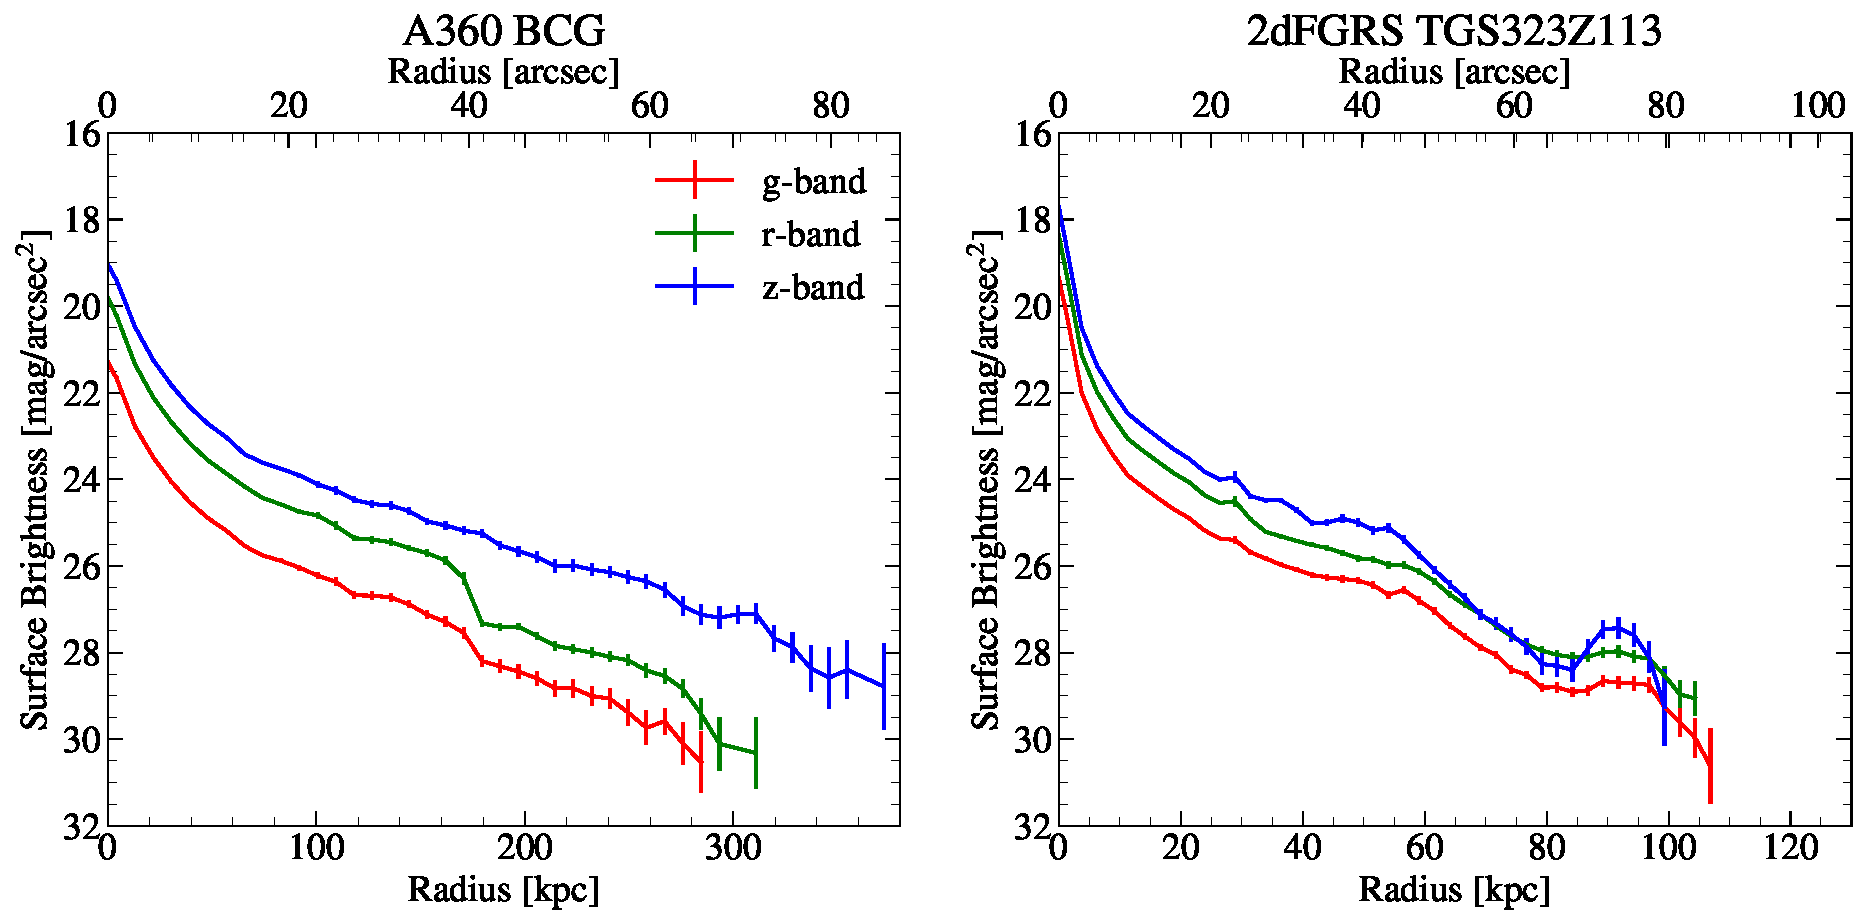
\includegraphics[width=1.0\linewidth]{figures/sb.pdf}
  \caption{The surface brightness profile in $g, r, z$ bands for the BCG of Abell 360 and 2dFGRS TGS323Z113. For both the BCG of Abell 360 and 2dFGRS TGS323Z113. The ComCam data can go as deep as 30 mag/arcsec$^2$ in the r-band.}
  \label{fig:sb}
\end{figure}

\section{Comparison with DECaLS}

In this section, we compare our ComCam measurement with the low surface brightness photometry from DECaLS with \textsc{legacyhalos}. We briefly describe the DECaLS measurement and refer readers to \cite{liReachingEdgeProbing2022,moustakasSienaGalaxyAtlas2023} for more details.  \lhalos first find CCDs that overlap in a 500kpc $\times$ 500kpc area on the sky. Then \lhalos builds a mosaic of the overlap with constant flux offsets added to each CCD image to ensure consistent backgrounds in between CCDs. For each CCD, we subtract the median sky background in a $[250, 275]$ kpc annulus at the redshift of the galaxy after masking out other sources in the annulus \citep{liReachingEdgeProbing2022}. We then project the background-subtracted images onto a tangent plane with Lanczos-3 interpolation kernel and build the image stack using inverse variance weighting. We then mask all sources identified by \textsc{The tractor} \citep{langTractorProbabilisticAstronomical2016} except for the massive galaxy of interest. We visually confirm that the unmasked region around the galaxy of interest is similar in DECaLS and ComCam data. With the masked image, we then use \textsc{photutils} to measure the surface brightness profile at a given major axis length with $3\sigma$ clipping of outlier clipping \citep{huangIndividualStellarHaloes2018, liReachingEdgeProbing2022}. In Figure~\ref{fig:comparison}, we show the comparison between of surface brightness profiles from ComCam data and DECaLS data. We see that the surface brightness profiles agree well between ComCam and DECaLS, and ComCam data can go deeper, especially in the $g$ band and $r$ band. 


\begin{figure}[!htbp]
  \centering
  % adjust width as you like (e.g. 0.8\linewidth, or specify height)
  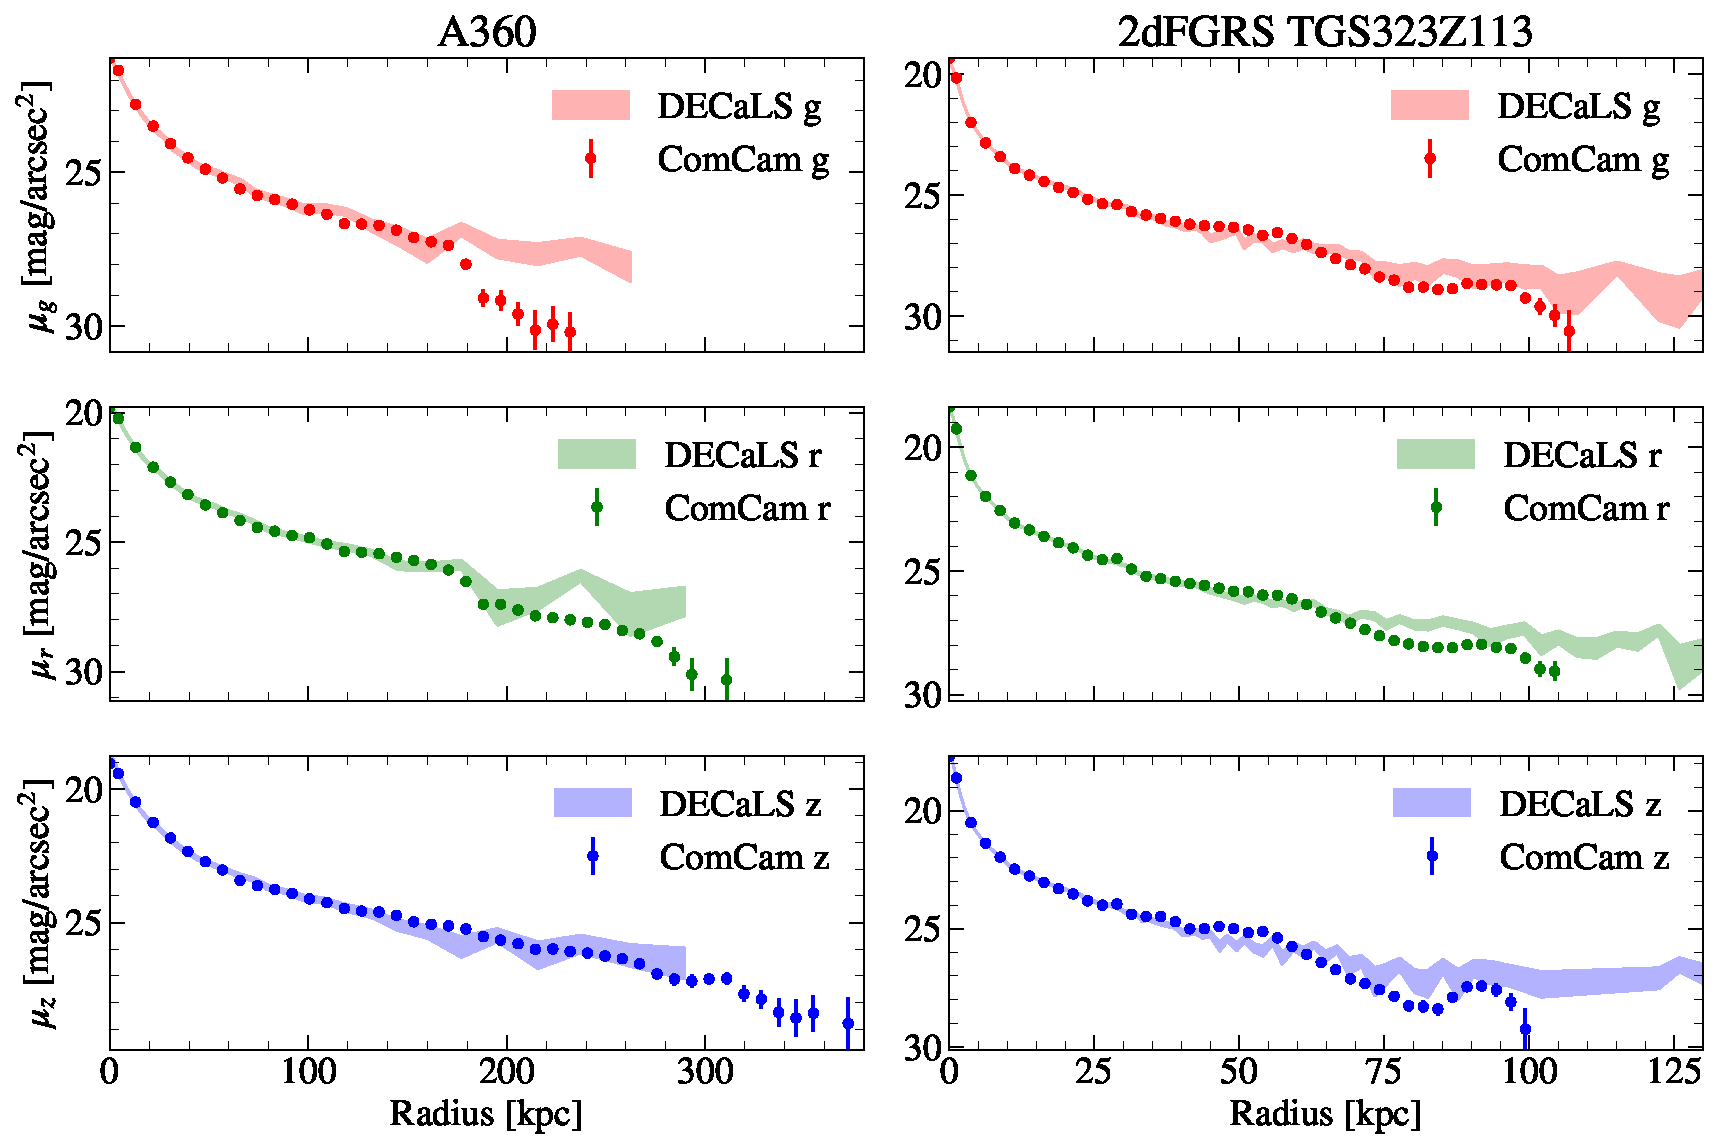
\includegraphics[width=1.0\linewidth]{figures/comparison.pdf}
  \caption{The comparison of surface rightness profiles from ComCam and DECaLS. The surface brightness profiles agree well in the center, while the ComCam data can go deeper in the outskirts.}
  \label{fig:comparison}
\end{figure}

\section{Conclusion}
In this technote, we perform elliptical isophote photometry on two galaxies with extended stellar halos in Rubin DP1 data and compare the results with photometry from DECaLS data. We find excellent agreement between the surface brightness profiles from Rubin DP1 and DECaLS at small radii, and the Rubin data can measure a lower surface brightness in the galaxy outskirt. 


\appendix
% Include all the relevant bib files.
% https://lsst-texmf.lsst.io/lsstdoc.html#bibliographies
\section{References} \label{sec:bib}
\renewcommand{\refname}{} % Suppress default Bibliography section
\bibliography{local,lsst,lsst-dm,refs_ads,refs,books,mylib}

% Make sure lsst-texmf/bin/generateAcronyms.py is in your path
\section{Acronyms} \label{sec:acronyms}
\addtocounter{table}{-1}
\begin{longtable}{p{0.145\textwidth}p{0.8\textwidth}}\hline
\textbf{Acronym} & \textbf{Description}  \\\hline

CCD & Charge-Coupled Device \\\hline
DECaLS & The Dark Energy Camera Legacy Survey \\\hline
DES & Dark Energy Survey \\\hline
DP1 & Data Preview 1 \\\hline
ECDFS & Extended Chandra Deep Field-South Survey \\\hline
LSST & Legacy Survey of Space and Time (formerly Large Synoptic Survey Telescope) \\\hline
LSSTComCam & Rubin Commissioning Camera \\\hline
NOAO & National Optical Astronomy Observatories now NOIRLab \\\hline
SE & System Engineering \\\hline
SV & Science Validation \\\hline
\end{longtable}

% If you want glossary uncomment below -- comment out the two lines above
%\printglossaries

\end{document}
